\documentclass[journal]{IEEEtran}
\usepackage[a5paper, margin=10mm, onecolumn]{geometry}
\usepackage{lmodern}
\usepackage{tfrupee}
\setlength{\headheight}{1cm}
\setlength{\headsep}{0mm}

\usepackage{gvv-book}
\usepackage{gvv}
\usepackage{cite}
\usepackage{amsmath,amssymb,amsfonts,amsthm}
\usepackage{algorithmic}
\usepackage{graphicx}
\usepackage{textcomp}
\usepackage{xcolor}
\usepackage{txfonts}
\usepackage{listings}
\usepackage{enumitem}
\usepackage{mathtools}
\usepackage{gensymb}
\usepackage{comment}
\usepackage[breaklinks=true]{hyperref}
\usepackage{tkz-euclide}
\usepackage{listings}
\def\inputGnumericTable{}
\usepackage[latin1]{inputenc}
\usepackage{color}
\usepackage{array}
\usepackage{longtable}
\usepackage{calc}
\usepackage{multirow}
\usepackage{hhline}
\usepackage{ifthen}
\usepackage{lscape}
\usepackage{xparse}

\bibliographystyle{IEEEtran}

\title{10.5.10}
\author{EE25BTECH11043 - Nishid Khandagre}

\begin{document}
\maketitle

\renewcommand{\thefigure}{\theenumi}
\renewcommand{\thetable}{\theenumi}

\numberwithin{equation}{enumi}
\numberwithin{figure}{enumi}

\textbf{Question}:\
Construct a tangent to a circle of radius 4 cm from a point which is at a distance of 6 cm from its centre.

\vspace{2mm}

\textbf{Solution:}
Let the center of the circle be the origin $\myvec{0\\0}$.
The equation of the circle with radius $R=4$ cm is:
\begin{align}
    \vec{C} \ : \ \vec{x}^{\top}\vec{V}\vec{x} + 2\vec{u}^{\top}\vec{x} + f=0 \ ; \ \vec{V}=\myvec{1&0\\0&1} \ , \ \vec{u}=\myvec{0\\0} \ , \ f=-R^2=-16
\end{align}
Let the external point from which the tangent is drawn be $\vec{h}$.
Given that the point is at a distance of 6 cm from the center, we can represent it as:
\begin{align}
    \vec{h}=\myvec{6\\0}
\end{align}

Now, calculate the matrix $\Sigma$:
\begin{align}
    \Sigma&=\brak{\vec{V}\vec{h} + \vec{u}}\brak{\vec{V}\vec{h} + \vec{u}}^{\top} - g\brak{\vec{h}}\vec{V}
    \end{align}
    \begin{align}
    g\brak{\vec{h}}=\vec{h}^{\top}\vec{V}\vec{h} + 2\vec{u}^{\top}\vec{h} + f = \norm{\vec{h}}^2 +f = 36 - 16 = 20
    \end{align}
    \begin{align}
    \Sigma&= \vec{h}\vec{h}^{\top} - g\brak{\vec{h}}\vec{V}\\
    &= \myvec{6 \\ 0}\myvec{6 & 0} - 20\myvec{ 1& 0 \\ 0 &1}\\
    &= \myvec{16 & 0 \\ 0 & -20}
\end{align}
The eigenvalues of $\Sigma$ are $\lambda_1=16$ and $\lambda_2=-20$.
The normalized eigenvectors form the matrix $\vec{P}$:
\begin{align}
    \vec{P}=\myvec{1 & 0\\0&1}
\end{align}
The direction vectors of the two tangents are given by:
\begin{align}
    \vec{m}=\vec{P}\myvec{\sqrt{\abs{\lambda_2}} \\ \pm\sqrt{\abs{\lambda_1}}} =\myvec{2\sqrt{5} \\ \pm 4}
\end{align}

The length of the tangent is given by
\begin{align}
    \norm{\vec{T}-\vec{h}}&=\abs{\mu} \norm{\vec{m}}
 \end{align}   
$\mu$ is a parameter
\begin{align}
    \mu&= -\dfrac{\vec{m}^{\top} \brak{\vec{V}\vec{h} + \vec{u}}}{\norm{\vec{m}}^2}=-\dfrac{\myvec{2\sqrt{5} & 4} \myvec{6\\0}}{\norm{\myvec{2\sqrt{5} \\ 4}}^2}=-\dfrac{\sqrt{5}}{3}
\end{align}
\begin{align}
    \norm{\vec{T}-\vec{h}}&=\dfrac{\sqrt{5}}{3} \times 6 \\
    &=2\sqrt{5} \approx 4.47 \text{ cm}
\end{align}

\begin{figure}[H]
\centering
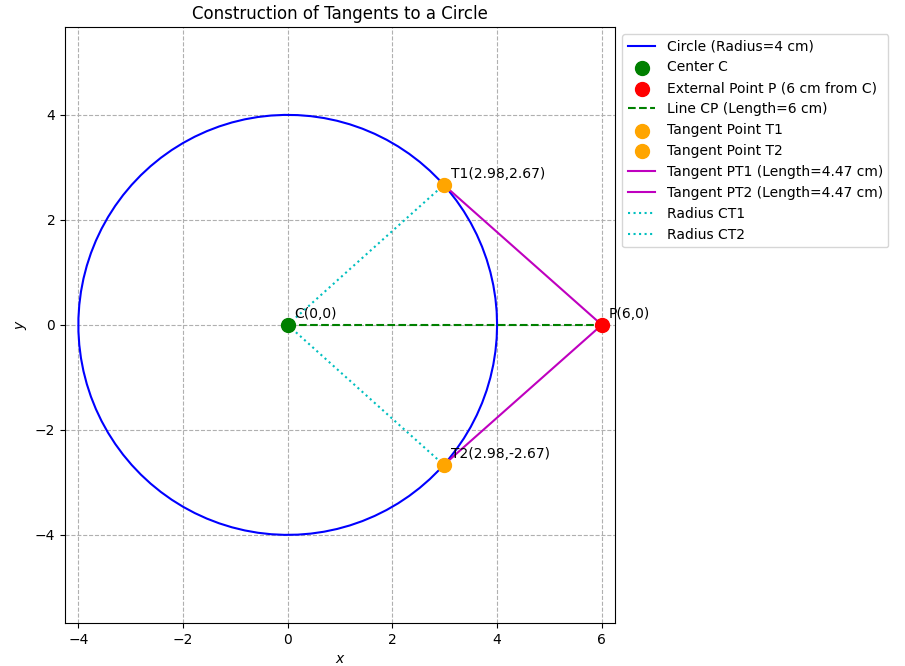
\includegraphics[width=0.9\columnwidth]{figs/fig1.png}
\caption{}
\label{fig:1}
\end{figure}

\end{document}
